\documentclass[aspectratio=169,11pt]{beamer}

\usepackage[T1]{fontenc}
\usepackage[utf8]{inputenc}
\usepackage{booktabs}
\usepackage{colortbl}
\usepackage{array}
\usepackage{amssymb}
\usepackage{tikz}
\usetikzlibrary{arrows.meta,positioning,shapes.geometric,calc,patterns}

% ---------- colours ----------
\definecolor{navy}{HTML}{1B2A4A}
\definecolor{teal}{HTML}{0E7C86}
\definecolor{amber}{HTML}{E8A33D}
\definecolor{coral}{HTML}{D9663F}
\definecolor{plum}{HTML}{7A4AA8}
\definecolor{leaf}{HTML}{3F9B5B}
\definecolor{bgtint}{HTML}{F2F6FA}
\definecolor{softteal}{HTML}{DDEFF0}
\definecolor{softamber}{HTML}{FBEBD0}

% ---------- standard Beamer theme ----------
\usetheme{Madrid}
\setbeamertemplate{navigation symbols}{}
\setbeamertemplate{blocks}[rounded][shadow=false]
\setbeamersize{text margin left=0.9cm,text margin right=0.9cm}
\setbeamercolor{background canvas}{bg=bgtint}
\setbeamercolor{normal text}{fg=navy!90!black}
\setbeamercolor{structure}{fg=teal}
\setbeamercolor{palette primary}{bg=navy,fg=white}
\setbeamercolor{palette secondary}{bg=teal,fg=white}
\setbeamercolor{palette tertiary}{bg=navy!80!black,fg=white}
\setbeamercolor{frametitle}{bg=navy,fg=white}
\setbeamercolor{title}{bg=navy,fg=white}
\setbeamercolor{block title}{bg=teal,fg=white}
\setbeamercolor{block body}{bg=softteal,fg=navy}
\setbeamercolor{block title alerted}{bg=coral,fg=white}
\setbeamercolor{block body alerted}{bg=coral!12,fg=navy}
\setbeamercolor{block title example}{bg=amber,fg=navy}
\setbeamercolor{block body example}{bg=softamber,fg=navy}
\setbeamercolor{itemize item}{fg=teal}
\setbeamercolor{enumerate item}{fg=teal}
\setbeamertemplate{itemize item}{$\blacktriangleright$}
\setbeamertemplate{enumerate item}{\insertenumlabel.}
\setbeamerfont{itemize/enumerate body}{size=\normalsize}
\setbeamerfont{block title}{size=\small}
\setbeamerfont{block body}{size=\small}

\newcommand{\why}[1]{\vspace{2pt}\begin{block}{Why}#1\end{block}}
\newcommand{\whys}[1]{\vspace{0pt}\begin{block}{Why}\scriptsize #1\end{block}}
\newcommand{\src}[1]{\par\vfill{\tiny\color{navy!60}Sources: #1}}
\renewcommand{\arraystretch}{1.25}

\tikzset{th/.style={draw=#1,thick,rounded corners=4pt,fill=white,text width=3.85cm,align=left,inner sep=5pt,minimum height=2.15cm}}
\tikzset{kb/.style={draw=#1,thick,rounded corners=4pt,fill=white,text width=6.35cm,align=left,inner sep=6pt,anchor=north west,minimum height=2.7cm}}
\tikzset{kh/.style={fill=#1,text=white,font=\bfseries\small,rounded corners=3pt,anchor=north west,inner sep=3pt,minimum width=6.35cm}}
\tikzset{bx/.style={draw=#1,thick,rounded corners=4pt,fill=white,align=center,inner sep=5pt,text width=2.5cm,minimum height=1.05cm}}
\tikzset{col/.style={draw=#1,thick,rounded corners=5pt,fill=white,text width=3.7cm,align=center,inner sep=6pt,minimum height=4.1cm,anchor=north}}
\tikzset{st/.style={draw=#1,thick,rounded corners=4pt,fill=white,align=center,inner sep=4pt,text width=3.4cm,minimum height=1.15cm}}

\tikzset{rqh/.style={fill=#1,text=white,font=\bfseries\footnotesize,rounded corners=3pt,text width=4.2cm,align=center,inner sep=4pt,anchor=north}}
\tikzset{chip/.style={fill=#1!12,draw=#1,thick,rounded corners=3pt,text width=3.9cm,minimum height=0.95cm,align=left,inner sep=4pt,font=\scriptsize,anchor=north}}

% paper card: colour, title, what they did, why it matters, what we take
\newcommand{\pcard}[5]{%
\begin{minipage}[t]{0.315\textwidth}
\setlength{\fboxsep}{5pt}
\colorbox{#1}{\parbox{\dimexpr\linewidth-10pt\relax}{\raggedright\small\bfseries\color{white}#2\strut}}\\[1pt]
\colorbox{white}{\parbox[t][3.95cm][t]{\dimexpr\linewidth-10pt\relax}{\raggedright\scriptsize
\textbf{\color{#1}What they did}\\#3\\[4pt]
\textbf{\color{#1}Why it matters}\\#4\\[4pt]
\textbf{\color{#1}What we take}\\#5}}
\end{minipage}}

\title[ML for ESG and Financial Risk]{Machine Learning for ESG Assessment and Financial Risk}
\subtitle{Literature, possible research questions and our plan}
\author[Singh, Gupta, Jaiswal]{Rajnish Singh \;$\cdot$\; Medhavie Gupta \;$\cdot$\; Katyayani Jaiswal}
\institute[GBU]{Gautam Buddha University, Greater Noida\\Guide: Prof.\ Valentina Lagasio, Sapienza University of Rome}
\date[20 Nov 2026]{Meeting on 20 November 2026}

\begin{document}

% ------------------------------------------------------------ 1 TITLE
\begin{frame}[plain]
\titlepage
\end{frame}

% ------------------------------------------------------------ 2 TEAM
\begin{frame}[t]{Who we are}
\centering
\begin{tikzpicture}[font=\small]
\foreach \x/\img/\name in {0/rajnish/Rajnish Singh, 4.8/medhavie/Medhavie Gupta, 9.6/katyayani/Katyayani Jaiswal}{
  \draw[rounded corners=5pt,teal,thick,fill=white] (\x,0.4) rectangle (\x+4.3,4.9);
  \fill[teal,rounded corners=5pt] (\x,4.3) rectangle (\x+4.3,4.9);
  \fill[teal] (\x,4.3) rectangle (\x+4.3,4.6);
  \begin{scope}
    \clip (\x+2.15,3.7) circle (0.9);
    \node at (\x+2.15,3.7) {\includegraphics[width=1.8cm]{\img_color.png}};
  \end{scope}
  \draw[amber,line width=1.6pt] (\x+2.15,3.7) circle (0.9);
  \node[font=\bfseries\normalsize,text=navy] at (\x+2.15,2.45) {\name};
  \node[anchor=north,text width=4.0cm,align=center,font=\footnotesize] at (\x+2.15,2.1) {B.Tech CSE, third year\\Gautam Buddha University\\Interest: AI and ML};
}
\draw[rounded corners=5pt,navy,fill=softamber,thick] (0,-1.15) rectangle (13.9,0.0);
\node[text width=13.2cm,align=center,font=\small] at (6.95,-0.57) {\textbf{Our guide: Prof.\ Valentina Lagasio}, Associate Professor in Financial Markets and Institutions,\\Department of Management, Faculty of Economics, Sapienza University of Rome};
\end{tikzpicture}
\end{frame}

% ------------------------------------------------------------ 3 AGENDA
\begin{frame}[t]{What we will cover}
\begin{columns}[T]
\column{0.55\textwidth}
\begin{enumerate}
\setlength{\itemsep}{5pt}
\item The problem and why it matters
\item Basic concepts (ESG, ML, SHAP, NLP)
\item Related work, paper by paper
\item Greenwashing and NLP papers
\item What the literature tells us
\item What may still be open
\item Our idea and eight possible research questions
\item Approach, data, plan and questions for you
\end{enumerate}
\column{0.42\textwidth}
\vspace{0.4cm}
\colorbox{softamber}{\parbox{0.95\textwidth}{\small
\textbf{Our goal today}\\[3pt]
Show what we read, share eight possible research questions, and get your advice on which direction to follow.\\[4pt]We are junior computer science students and finance is new to us, so your guidance matters.}}
\end{columns}
\end{frame}

\section{The problem}
% ------------------------------------------------------------ 4 PROBLEM
\begin{frame}[t]{The problem: ESG ratings are hard to trust}
\begin{columns}[T]
\column{0.5\textwidth}
\setbeamerfont{itemize/enumerate body}{size=\footnotesize}
\footnotesize
\begin{itemize}
\setlength{\itemsep}{1pt}
\item The same company gets \textbf{different ESG scores} from different rating agencies (Berg et al., 2022).
\item ESG data is \textbf{often missing}, and distressed firms are less likely to be rated (Raza et al., 2026).
\item Machine learning can predict ESG scores well (Zhang and Zhao, 2026), but most studies we read give \textbf{one number}, not how sure the model is.
\item Firms can also \textbf{sound greener than they are} (greenwashing).
\end{itemize}
\column{0.48\textwidth}
\centering
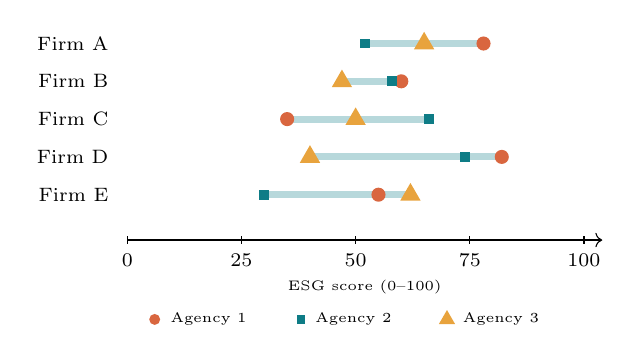
\begin{tikzpicture}[x=0.058cm,y=0.48cm,font=\scriptsize]
\draw[->] (0,0.2) -- (104,0.2);
\foreach \v in {0,25,50,75,100}{\draw (\v,0.1) -- (\v,0.3); \node[anchor=north] at (\v,0.1) {\v};}
\node[anchor=north,font=\tiny] at (52,-0.6) {ESG score (0--100)};
\foreach \y/\n/\a/\b/\c in {5/Firm A/78/52/65, 4/Firm B/60/58/47, 3/Firm C/35/66/50, 2/Firm D/82/74/40, 1/Firm E/55/30/62}{
  \node[anchor=east] at (-2,\y+0.4) {\n};
  \draw[teal!30,line width=2.6pt] ({min(\a,min(\b,\c))},\y+0.4) -- ({max(\a,max(\b,\c))},\y+0.4);
  \node[circle,fill=coral,inner sep=1.8pt] at (\a,\y+0.4) {};
  \node[rectangle,fill=teal,inner sep=1.8pt] at (\b,\y+0.4) {};
  \node[regular polygon,regular polygon sides=3,fill=amber,inner sep=1.5pt] at (\c,\y+0.4) {};
}
\node[circle,fill=coral,inner sep=1.4pt,label=right:{\tiny Agency 1}] at (6,-1.9) {};
\node[rectangle,fill=teal,inner sep=1.5pt,label=right:{\tiny Agency 2}] at (38,-1.9) {};
\node[regular polygon,regular polygon sides=3,fill=amber,inner sep=1.2pt,label=right:{\tiny Agency 3}] at (70,-1.9) {};
\end{tikzpicture}

{\tiny\color{navy!60}Illustrative numbers, not real data. The light bar shows the spread.}
\end{columns}
\whys{If scores disagree and are incomplete, decisions built on them are shaky.}
\end{frame}

% ------------------------------------------------------------ 5 SOURCES OF DISAGREEMENT
\begin{frame}[t]{Where does the disagreement come from?}
\begin{columns}[T]
\column{0.5\textwidth}
Berg et al.\ (2022) split the disagreement between rating agencies into three parts:
\begin{itemize}
\setlength{\itemsep}{2pt}
\item \textbf{Scope:} which topics are included.
\item \textbf{Measurement:} how each topic is measured.
\item \textbf{Weight:} how important each topic is.
\end{itemize}
They report that measurement is the largest part, scope is second, and weight is the smallest.
\why{The problem is not only opinion. Data and measurement are noisy, and this is where ML and uncertainty tools can help.}
\column{0.48\textwidth}
\vspace{0.3cm}
\centering
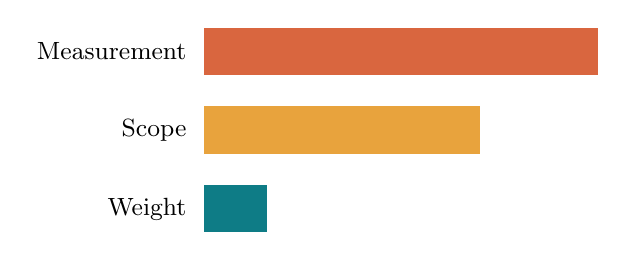
\begin{tikzpicture}[font=\small]
\fill[coral] (0,2.2) rectangle (5.0,2.8);
\fill[amber] (0,1.2) rectangle (3.5,1.8);
\fill[teal] (0,0.2) rectangle (0.8,0.8);
\node[anchor=east] at (-0.1,2.5) {Measurement};
\node[anchor=east] at (-0.1,1.5) {Scope};
\node[anchor=east] at (-0.1,0.5) {Weight};
\end{tikzpicture}

{\tiny\color{navy!60}Schematic: relative size only (Berg et al., 2022). Exact shares differ between versions of the paper.}
\end{columns}
\src{Berg, K\"olbel and Rigobon (2022), Review of Finance.}
\end{frame}

% ------------------------------------------------------------ 6 IMPACT
\begin{frame}[t]{Why it matters: who is affected?}
\begin{columns}[T]
\column{0.32\textwidth}
\textbf{\color{coral}Investors}\\[3pt]
They use ESG scores to choose investments. A finance model shows that uncertainty about ESG ratings changes how investors build portfolios (Avramov et al., 2022).
\column{0.32\textwidth}
\textbf{\color{teal}Banks and lenders}\\[3pt]
ESG information is linked to credit decisions. But ESG scores are not standardised, and ML models can lack explainability (Giudici and Wu, 2025).
\column{0.32\textwidth}
\textbf{\color{plum}Companies and regulators}\\[3pt]
Mixed signals make it hard to compare firms fairly. Regulators also act against misleading green claims; the UK FCA anti-greenwashing rule started in May 2024 (UK greenwashing study, 2026).
\end{columns}
\vspace{10pt}
\why{A score is only useful if people know how far to rely on it. Showing the uncertainty, and checking the text behind it, is a practical step towards that.}
\src{Avramov, Cheng, Lioui and Tarelli (2022); Giudici and Wu (2025); UK greenwashing study (2026, Zenodo).}
\end{frame}

\section{Concepts}
% ------------------------------------------------------------ 7 CONCEPTS
\begin{frame}[t]{Basic concepts we are using}
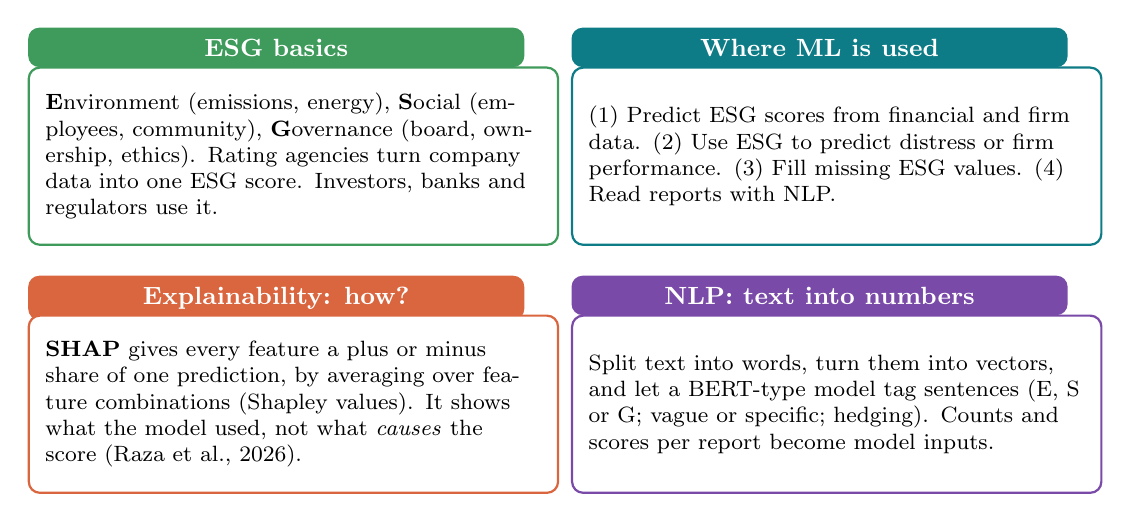
\begin{tikzpicture}[font=\footnotesize]
\tikzset{cb/.style={draw=none,rounded corners=4pt,fill=white,text width=6.3cm,align=left,inner sep=6pt,minimum height=2.25cm,anchor=north west}}
\tikzset{hd/.style={rounded corners=4pt,text=white,font=\bfseries\small,anchor=north west,inner sep=4pt,minimum width=6.3cm}}
\node[hd,fill=leaf] at (0,0) {ESG basics};
\node[cb,draw=leaf,thick] at (0,-0.5) {\textbf{E}nvironment (emissions, energy), \textbf{S}ocial (employees, community), \textbf{G}overnance (board, ownership, ethics). Rating agencies turn company data into one ESG score. Investors, banks and regulators use it.};
\node[hd,fill=teal] at (6.9,0) {Where ML is used};
\node[cb,draw=teal,thick] at (6.9,-0.5) {(1) Predict ESG scores from financial and firm data. (2) Use ESG to predict distress or firm performance. (3) Fill missing ESG values. (4) Read reports with NLP.};
\node[hd,fill=coral] at (0,-3.15) {Explainability: how?};
\node[cb,draw=coral,thick] at (0,-3.65) {\textbf{SHAP} gives every feature a plus or minus share of one prediction, by averaging over feature combinations (Shapley values). It shows what the model used, not what \emph{causes} the score (Raza et al., 2026).};
\node[hd,fill=plum] at (6.9,-3.15) {NLP: text into numbers};
\node[cb,draw=plum,thick] at (6.9,-3.65) {Split text into words, turn them into vectors, and let a BERT-type model tag sentences (E, S or G; vague or specific; hedging). Counts and scores per report become model inputs.};
\end{tikzpicture}
\end{frame}

\section{Related work}
% ------------------------------------------------------------ 8 RELATED WORK MAP
\begin{frame}[t]{Related work: what we read}
\centering
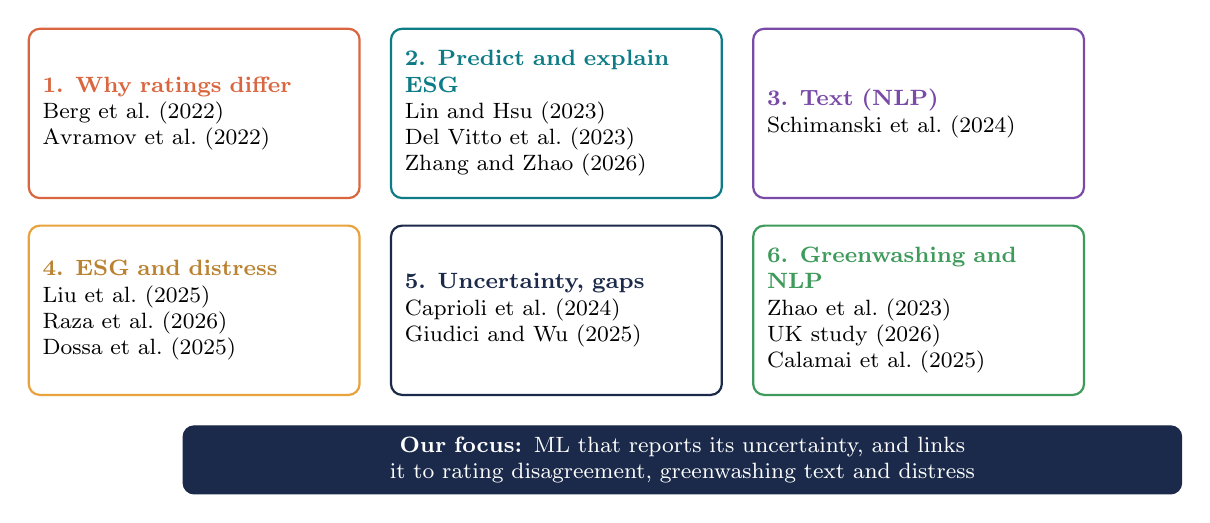
\begin{tikzpicture}[font=\footnotesize]
\node[th=coral] (a) at (0,0) {\textbf{\color{coral}1. Why ratings differ}\\Berg et al.\ (2022)\\Avramov et al.\ (2022)};
\node[th=teal] (b) at (4.6,0) {\textbf{\color{teal}2. Predict and explain ESG}\\Lin and Hsu (2023)\\Del Vitto et al.\ (2023)\\Zhang and Zhao (2026)};
\node[th=plum] (c) at (9.2,0) {\textbf{\color{plum}3. Text (NLP)}\\Schimanski et al.\ (2024)};
\node[th=amber] (d) at (0,-2.5) {\textbf{\color{amber!80!black}4. ESG and distress}\\Liu et al.\ (2025)\\Raza et al.\ (2026)\\Dossa et al.\ (2025)};
\node[th=navy] (e) at (4.6,-2.5) {\textbf{\color{navy}5. Uncertainty, gaps}\\Caprioli et al.\ (2024)\\Giudici and Wu (2025)};
\node[th=leaf] (g) at (9.2,-2.5) {\textbf{\color{leaf}6. Greenwashing and NLP}\\Zhao et al.\ (2023)\\UK study (2026)\\Calamai et al.\ (2025)};
\node[draw=navy,fill=navy,rounded corners=4pt,text=white,text width=12.4cm,align=center,inner sep=4pt] at (6.2,-4.4) {\textbf{Our focus:} ML that reports its uncertainty, and links it to rating disagreement, greenwashing text and distress};
\end{tikzpicture}
\src{Papers listed in the references. Based on abstracts, publisher pages and, for some, full text; we are reading the rest.}
\end{frame}

% ------------------------------------------------------------ 9 CORE 1
\begin{frame}[t]{Core papers (1/3): predicting and explaining ESG scores}
\pcard{teal}{Lin and Hsu (2023)\\{\scriptsize\mdseries Taiwan, \emph{Sustainability}}}
{Uses ML models to predict ESG scores of non-financial firms in Taiwan from firm data.}
{An ESG score can be estimated from public firm data, so gaps can be filled.}
{A simple recipe: data, train, test, compare models.}
\hfill
\pcard{coral}{Del Vitto et al.\ (2023)\\{\scriptsize\mdseries \emph{Annals of Operations Research}}}
{Uses ML techniques to explain how ESG ratings come about, not only to predict them.}
{A rating that cannot be explained is hard to trust or challenge.}
{How to open the black box and show which inputs drive a rating.}
\hfill
\pcard{plum}{Zhang and Zhao (2026)\\{\scriptsize\mdseries China A-shares, 2013--2022}}
{XGBoost with SHAP predicts corporate ESG ratings; reported accuracy 91.0\%.}
{A strong and explainable result, but it gives one predicted rating, no uncertainty range.}
{Our baseline model. We then add uncertainty on top.}
\whys{All three predict or explain ESG with ML, each on one market. They are our starting point for RQ1 and RQ7.}
\end{frame}

% ------------------------------------------------------------ 10 CORE 2
\begin{frame}[t]{Core papers (2/3): disagreement, uncertainty, text}
\pcard{coral}{Berg et al.\ (2022)\\{\scriptsize\mdseries \emph{Review of Finance}}}
{Compares ratings of six agencies; splits disagreement into scope, measurement, weight.}
{Measurement is the largest part: noisy data drives disagreement.}
{The disagreement problem, and where ML can help.}
\hfill
\pcard{teal}{Avramov et al.\ (2022)\\{\scriptsize\mdseries \emph{Journal of Financial Economics}}}
{A finance model of investing when ESG ratings are uncertain.}
{Uncertainty about ratings changes how investors build portfolios.}
{A reason to estimate uncertainty and to test if it carries information.}
\hfill
\pcard{plum}{Schimanski et al.\ (2024)\\{\scriptsize\mdseries \emph{Finance Research Letters}}}
{Uses NLP to measure environmental, social and governance communication in text.}
{Turns reports into ESG-text numbers that can sit beside financial numbers.}
{Text features for RQ3, RQ4 and RQ5.}
\whys{Problem (Berg), reason to care (Avramov), and a tool for the text side (Schimanski).}
\end{frame}

% ------------------------------------------------------------ 11 CORE 3
\begin{frame}[t]{Core papers (3/3): ESG, distress, performance}
\pcard{amber!85!black}{Liu et al.\ (2025)\\{\scriptsize\mdseries \emph{Int.\ J.\ of Finance and Economics}}}
{ESG-driven deep learning to predict financial distress, with risk-based stratification of firms.}
{Treats ESG as an input for financial risk, which is close to our RQ2.}
{The distress set-up. We compare it with simpler models.}
\hfill
\pcard{navy}{Raza et al.\ (2026)\\{\scriptsize\mdseries 12 Asia-Pacific markets}}
{47,253 firm-years, tested on later years only. Also checks ESG controversies.}
{No extra predictive value from ESG once financial ratios are in; coverage is selective.}
{A strict out-of-time test, and a warning that we must show real added value.}
\hfill
\pcard{leaf}{Dossa et al.\ (2025)\\{\scriptsize\mdseries \emph{Innovation and Green Development}}}
{ML with explainability tools on the link between ESG disclosure and firm performance.}
{Extra Trees worked best. Disclosure is positively linked with performance, most for environmental.}
{A pillar-wise view (E, S, G) for RQ6; tree models suit firm data.}
\whys{Evidence on ESG and financial outcomes is mixed (Raza vs.\ Dossa), so testing on later years matters.}
\end{frame}

% ------------------------------------------------------------ 12 MORE RECENT
\begin{frame}[t]{Related work: more recent studies}
\small
\begin{itemize}
\setlength{\itemsep}{7pt}
\item \textbf{Giudici and Wu (2025):} uses ensemble ML and Shapley values to study how ESG scores relate to credit ratings. \emph{We take:} explainability and robustness checks.
\item \textbf{Caprioli et al.\ (2024, preprint):} compares ML methods to fill missing ESG data and gives prediction intervals. \emph{We take:} ways to show uncertainty.
\item \textbf{Cheng et al.\ (2025); Wu et al.\ (2025):} combine ML with ESG divergence in Hong Kong and China. \emph{We take:} divergence and ML are active topics, but these studies use one market each.
\end{itemize}
\why{These papers show that our topic is current, and that explainability and uncertainty are both wanted by the field.}
\src{Giudici and Wu (2025); Caprioli et al.\ (2024); Cheng et al.\ (2025); Wu et al.\ (2025).}
\end{frame}

% ------------------------------------------------------------ 13 GREENWASHING PAPERS
\begin{frame}[t]{Greenwashing and NLP: three papers}
\pcard{leaf}{Zhao et al.\ (2023)\\{\scriptsize\mdseries KDIR conference, pp.\ 175--181}}
{NLP on internal documents and social media of 12 pharma firms, 2012--2022; compares internal and public ESG sentiment.}
{No significant link between the two; a mismatch may point to greenwashing.}
{A text-versus-outside-view idea. Small sample, so a pilot only.}
\hfill
\pcard{amber!85!black}{UK study (2026)\\{\scriptsize\mdseries Zenodo record, 31 Jan 2026}}
{487 UK firms, 2018--2024. NLP on reports (86.34\% accuracy) plus XGBoost and Random Forest on ESG-financial gaps.}
{Firm size, governance and financial constraints predict greenwashing.}
{Text plus numbers in one study. Not peer reviewed, so we verify it.}
\hfill
\pcard{plum}{Calamai et al.\ (2025)\\{\scriptsize\mdseries arXiv survey, v2 Jan 2026}}
{Surveys NLP for greenwashing: ESG tagging, green claims, sentiment, deception, stance.}
{Some subtasks look solved, but a reliable full detector is still open.}
{A map of which text tasks to use, and what is still hard.}
\whys{Links to your ESG-washing research. Mostly text-based; links to ratings and distress need checking.}
\end{frame}

% ------------------------------------------------------------ 14 KEY FINDINGS
\begin{frame}[t]{What the literature tells us}
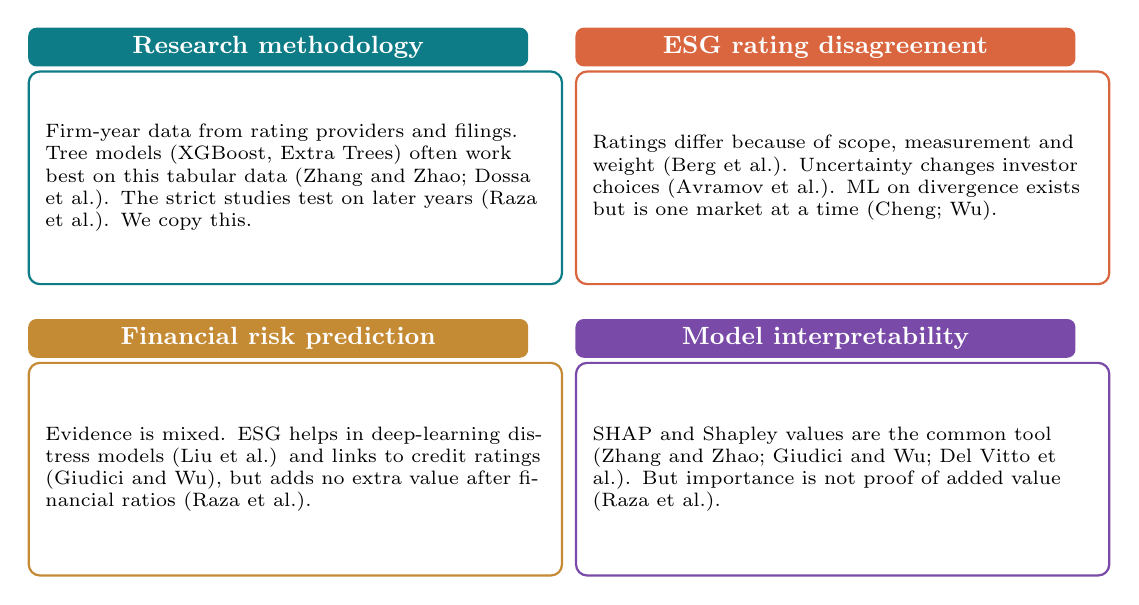
\begin{tikzpicture}[font=\scriptsize]
\node[kh=teal] at (0,0) {Research methodology};
\node[kb=teal] at (0,-0.55) {Firm-year data from rating providers and filings. Tree models (XGBoost, Extra Trees) often work best on this tabular data (Zhang and Zhao; Dossa et al.). The strict studies test on later years (Raza et al.). We copy this.};
\node[kh=coral] at (6.95,0) {ESG rating disagreement};
\node[kb=coral] at (6.95,-0.55) {Ratings differ because of scope, measurement and weight (Berg et al.). Uncertainty changes investor choices (Avramov et al.). ML on divergence exists but is one market at a time (Cheng; Wu).};
\node[kh=amber!85!black] at (0,-3.7) {Financial risk prediction};
\node[kb=amber!85!black] at (0,-4.25) {Evidence is mixed. ESG helps in deep-learning distress models (Liu et al.) and links to credit ratings (Giudici and Wu), but adds no extra value after financial ratios (Raza et al.).};
\node[kh=plum] at (6.95,-3.7) {Model interpretability};
\node[kb=plum] at (6.95,-4.25) {SHAP and Shapley values are the common tool (Zhang and Zhao; Giudici and Wu; Del Vitto et al.). But importance is not proof of added value (Raza et al.).};
\end{tikzpicture}
\end{frame}

\section{Gaps and idea}
% ------------------------------------------------------------ 15 OPEN QUESTIONS
\begin{frame}[t]{What may still be open (we are verifying)}
\scriptsize\renewcommand{\arraystretch}{1.1}
\begin{tabular}{@{}p{0.5cm}p{6.1cm}p{6.6cm}@{}}
\toprule
\rowcolor{softteal}\color{navy} & \color{navy}Possible open question & \color{navy}What we saw so far \\
\midrule
1 & Uncertainty and prediction are often studied apart & Rating-uncertainty papers are finance models (Berg; Avramov); ML score papers give point predictions (Lin and Hsu; Zhang and Zhao) \\
2 & Does ESG help predict distress? Evidence is not settled & Raza et al.\ find no extra value once financials are included; Liu et al.\ and Dossa et al.\ find useful links \\
3 & Many ML studies use one market & Taiwan, China, Hong Kong samples (Lin and Hsu; Zhang and Zhao; Cheng; Wu) \\
4 & ESG coverage is selective & Distressed firms are less likely to be rated (Raza et al.) \\
5 & Do text and numbers tell the same story? & NLP can measure ESG communication (Schimanski); greenwashing studies compare text with outside views (Zhao; UK 2026) \\
6 & Is greenwashing linked to rating disagreement and distress? & Calamai et al.\ say reliable detection is still open; we must check if links to ratings and distress are studied \\
\bottomrule
\end{tabular}
\why{We do not claim novelty yet. Each point will be checked against more literature.}
\end{frame}

% ------------------------------------------------------------ 16 PROPOSED IDEA
\begin{frame}[t]{Proposed idea: ESG models that show uncertainty}
\begin{center}
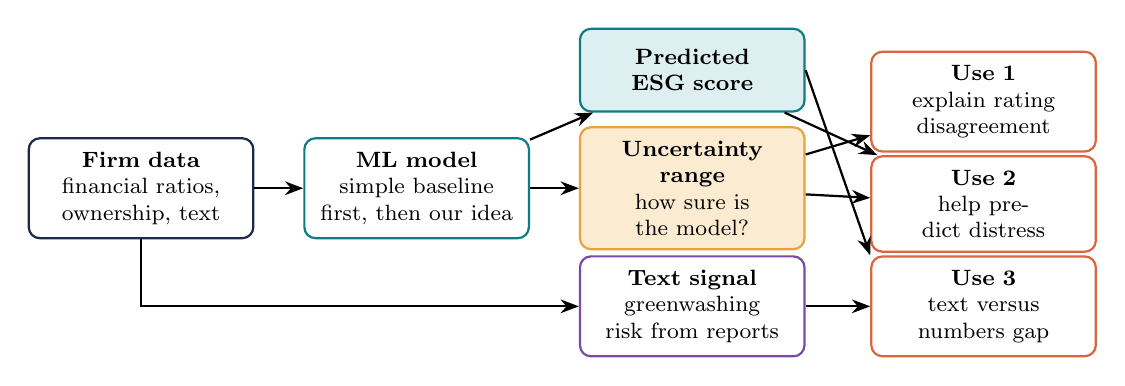
\begin{tikzpicture}[font=\footnotesize,>=Stealth]
\node[bx=navy] (n1) at (0,0) {\textbf{Firm data}\\financial ratios, ownership, text};
\node[bx=teal] (n2) at (3.5,0) {\textbf{ML model}\\simple baseline first, then our idea};
\node[bx=teal,fill=softteal] (n3) at (7.0,1.5) {\textbf{Predicted ESG score}};
\node[bx=amber,fill=softamber] (n4) at (7.0,0) {\textbf{Uncertainty range}\\how sure is the model?};
\node[bx=plum] (n7) at (7.0,-1.5) {\textbf{Text signal}\\greenwashing risk from reports};
\node[bx=coral] (n5) at (10.7,1.1) {\textbf{Use 1}\\explain rating disagreement};
\node[bx=coral] (n6) at (10.7,-0.2) {\textbf{Use 2}\\help predict distress};
\node[bx=coral] (n8) at (10.7,-1.5) {\textbf{Use 3}\\text versus numbers gap};
\draw[->,thick] (n1) -- (n2);
\draw[->,thick] (n2) -- (n3); \draw[->,thick] (n2) -- (n4);
\draw[->,thick] (n1.south) |- (n7.west);
\draw[->,thick] (n4) -- (n5); \draw[->,thick] (n4) -- (n6); \draw[->,thick] (n3) -- (n6);
\draw[->,thick] (n7) -- (n8); \draw[->,thick] (n3.east) -- (n8.north west);
\end{tikzpicture}
\end{center}
\vspace{-4pt}
\why{Rating uncertainty (Berg; Avramov), ML score prediction (Lin and Hsu; Zhang and Zhao) and greenwashing text (Zhao; Calamai) seem studied apart. We want to join them and test if uncertainty and text carry useful information.}
\end{frame}

\section{Research questions}
% ------------------------------------------------------------ 17 RQ MAP
\begin{frame}[t]{Eight possible research questions: three themes}
\begin{center}
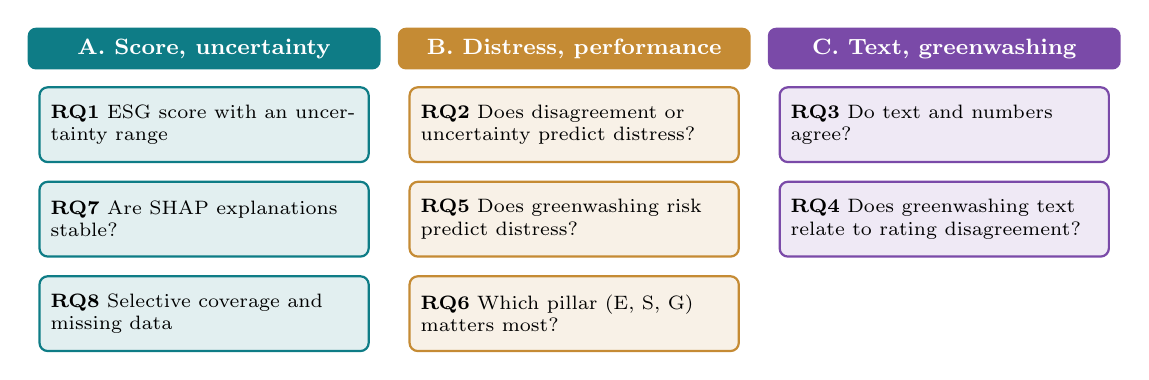
\begin{tikzpicture}[font=\footnotesize]
\node[rqh=teal] at (0,0) {A. Score, uncertainty};
\node[chip=teal] at (0,-0.75) {\textbf{RQ1} ESG score with an uncertainty range};
\node[chip=teal] at (0,-1.95) {\textbf{RQ7} Are SHAP explanations stable?};
\node[chip=teal] at (0,-3.15) {\textbf{RQ8} Selective coverage and missing data};
\node[rqh=amber!85!black] at (4.7,0) {B. Distress, performance};
\node[chip=amber!85!black] at (4.7,-0.75) {\textbf{RQ2} Does disagreement or uncertainty predict distress?};
\node[chip=amber!85!black] at (4.7,-1.95) {\textbf{RQ5} Does greenwashing risk predict distress?};
\node[chip=amber!85!black] at (4.7,-3.15) {\textbf{RQ6} Which pillar (E, S, G) matters most?};
\node[rqh=plum] at (9.4,0) {C. Text, greenwashing};
\node[chip=plum] at (9.4,-0.75) {\textbf{RQ3} Do text and numbers agree?};
\node[chip=plum] at (9.4,-1.95) {\textbf{RQ4} Does greenwashing text relate to rating disagreement?};
\end{tikzpicture}
\end{center}
\why{RQ4 and RQ5 connect the text theme with the other two. We expect to keep a small bundle of these after your advice.}
\end{frame}

% ------------------------------------------------------------ 18 RQ 1-4
\begin{frame}[t]{Research questions (1/2): preliminary}
\scriptsize
\begin{tabular}{@{}p{0.9cm}p{5.0cm}p{3.7cm}p{3.5cm}@{}}
\toprule
\rowcolor{softteal} & \textbf{Question} & \textbf{Why we ask} & \textbf{Main reading} \\
\midrule
\textbf{\color{teal}RQ1} & Can ML predict ESG scores \textbf{with a reliable uncertainty range}? & Scores without ranges hide risk & Zhang and Zhao (2026); Caprioli et al.\ (2024) \\
\textbf{\color{amber!85!black}RQ2} & Does ESG \textbf{disagreement or uncertainty} help predict financial distress beyond financial ratios, on later years? & ESG level alone adds little (Raza); uncertainty may carry more & Raza et al.\ (2026); Berg et al.\ (2022) \\
\textbf{\color{plum}RQ3} & Do firms' \textbf{reports (text) and numbers} tell the same ESG story? & A gap may signal ESG-washing & Schimanski et al.\ (2024); Zhao et al.\ (2023) \\
\textbf{\color{plum}RQ4} & Does a \textbf{text-based greenwashing score} relate to disagreement between ESG rating agencies? & Vague text may explain part of the measurement disagreement & Berg et al.\ (2022); Calamai et al.\ (2025) \\
\bottomrule
\end{tabular}
\why{These are preliminary and may fail. A negative result is still a result.}
\end{frame}

% ------------------------------------------------------------ 19 RQ 5-8
\begin{frame}[t]{Research questions (2/2): preliminary}
\scriptsize
\begin{tabular}{@{}p{0.9cm}p{5.0cm}p{3.7cm}p{3.5cm}@{}}
\toprule
\rowcolor{softteal} & \textbf{Question} & \textbf{Why we ask} & \textbf{Main reading} \\
\midrule
\textbf{\color{amber!85!black}RQ5} & Does \textbf{greenwashing risk} help predict financial distress beyond financial ratios? & Misleading disclosure may hide risk; UK study links gaps to firm traits & UK study (2026); Raza et al.\ (2026); Liu et al.\ (2025) \\
\textbf{\color{amber!85!black}RQ6} & Which pillar, \textbf{E, S or G}, matters most for firm performance, and does it hold on later years? & Dossa et al.\ find environmental strongest; we test out of time & Dossa et al.\ (2025); Giudici and Wu (2025) \\
\textbf{\color{teal}RQ7} & Are \textbf{SHAP explanations stable} across models, years and markets? & Explanations should not change with small choices; many studies use one market & Del Vitto et al.\ (2023); Zhang and Zhao (2026); Cheng; Wu \\
\textbf{\color{teal}RQ8} & Does \textbf{selective ESG coverage} bias results, and do uncertainty-aware fills of missing data help? & Distressed firms are less likely to be rated & Raza et al.\ (2026); Caprioli et al.\ (2024) \\
\bottomrule
\end{tabular}
\why{We will keep one or two (or a small bundle such as RQ1 with RQ2) after we check the literature and hear your advice.}
\end{frame}

% ------------------------------------------------------------ 19b CONSOLIDATED CORE RQS
\begin{frame}[t]{Consolidated Core Research Questions}
\small
\begin{block}{\textbf{Question 1: Rating Divergence, Harmonization \& Financial Risk}}
\textbf{How do differences in rating agency methodologies and disclosure standards drive ESG rating divergence, and how would aligning ratings around common reporting frameworks or standardized baselines affect rating consistency and financial risk assessment?}
\vspace{3pt}
\begin{itemize}\setlength{\itemsep}{1pt}
  \item \textbf{Divergence Drivers:} Measurement error (56\%), scope differences (38\%), and weighting discrepancies (6\%) (Berg et al., 2022).
  \item \textbf{Harmonization Effect:} Impact of transitioning from voluntary CSR to statutory baselines (UK SECR / TCFD).
  \item \textbf{Financial Risk:} Incremental predictive value for out-of-time credit spreads and insolvency forecasting.
\end{itemize}
\end{block}
\vspace{3pt}
\begin{exampleblock}{\textbf{Question 2: Transformer Models \& ESG-Washing Discrepancy Detection}}
\textbf{How can state-of-the-art transformer models (like BERT) and sentiment analysis be deployed to detect corporate ESG-washing and evaluate reporting discrepancies?}
\vspace{3pt}
\begin{itemize}\setlength{\itemsep}{1pt}
  \item \textbf{Contextual NLP:} Benchmarking FinBERT / ClimateBERT vs.\ classical lexicons for disclosure sentiment polarity.
  \item \textbf{Discrepancy Formulation:} Objective gap metric between narrative disclosure tone and verified carbon/CapEx metrics.
  \item \textbf{Risk Linkage:} Correlation with multi-agency rating disagreement ($r=0.443$) and early-warning distress signals.
\end{itemize}
\end{exampleblock}
\end{frame}

\section{Approach and plan}
% ------------------------------------------------------------ 20 APPROACH
\begin{frame}[t]{Our approach}
\begin{center}
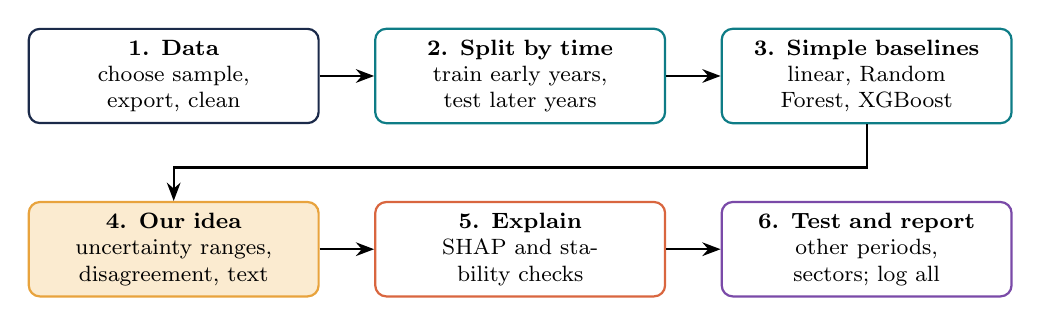
\begin{tikzpicture}[font=\footnotesize,>=Stealth]
\node[st=navy] (a) at (0,0) {\textbf{1. Data}\\choose sample, export, clean};
\node[st=teal] (b) at (4.4,0) {\textbf{2. Split by time}\\train early years, test later years};
\node[st=teal] (c) at (8.8,0) {\textbf{3. Simple baselines}\\linear, Random Forest, XGBoost};
\node[st=amber,fill=softamber] (d) at (0,-2.2) {\textbf{4. Our idea}\\uncertainty ranges, disagreement, text};
\node[st=coral] (e) at (4.4,-2.2) {\textbf{5. Explain}\\SHAP and stability checks};
\node[st=plum] (f) at (8.8,-2.2) {\textbf{6. Test and report}\\other periods, sectors; log all};
\draw[->,thick] (a) -- (b); \draw[->,thick] (b) -- (c);
\draw[->,thick] (c.south) -- ++(0,-0.55) -| (d.north);
\draw[->,thick] (d) -- (e); \draw[->,thick] (e) -- (f);
\end{tikzpicture}
\end{center}
\vspace{-2pt}
\why{Simple first, one change at a time, and always test on future years. We use complex models only if they clearly help.}
\end{frame}

% ------------------------------------------------------------ 21 METHODS WITH REASONS
\begin{frame}[t]{Methods and the reasons behind them}
\scriptsize
\begin{tabular}{@{}p{2.3cm}p{5.0cm}p{5.9cm}@{}}
\toprule
\rowcolor{softteal} \textbf{Step} & \textbf{What we will do} & \textbf{Why (source)} \\
\midrule
Test design & Train on early years, test on later years; keep some firms unseen & Raza et al.\ (2026) use a strict out-of-time test \\
Baselines & Linear or logistic, Random Forest, XGBoost, Extra Trees & Simple first; XGBoost with SHAP predicted ESG ratings well (Zhang and Zhao, 2026); Extra Trees did best in Dossa et al.\ (2025) \\
Uncertainty & Bootstrap, quantile models, conformal ranges & Prediction intervals show how sure a model is (Caprioli et al., 2024) \\
Explain & SHAP, plus a check that a feature really improves future predictions & SHAP importance is not proof of added value (Raza et al., 2026); explainability is needed (Giudici and Wu, 2025) \\
Text (if needed) & ESG-BERT-type models, hedging and vagueness scores on reports & NLP can measure ESG communication (Schimanski et al., 2024); greenwashing signals (Zhao et al., 2023; Calamai et al., 2025) \\
Deep learning & Only if it clearly beats simpler models & Keeps results explainable and fair to compare \\
\bottomrule
\end{tabular}
\src{Raza et al.\ (2026); Zhang and Zhao (2026); Dossa et al.\ (2025); Caprioli et al.\ (2024); Giudici and Wu (2025); Schimanski et al.\ (2024); Zhao et al.\ (2023); Calamai et al.\ (2025).}
\end{frame}

% ------------------------------------------------------------ 22 DATA
\begin{frame}[t]{Data: Orbis and what we still need}
\begin{columns}[T]
\column{0.52\textwidth}
\setbeamerfont{itemize/enumerate body}{size=\scriptsize}
\footnotesize
\textbf{Orbis (as you described it) gives:}
\begin{itemize}
\setlength{\itemsep}{1pt}
\item Company financials over many years
\item Ownership and group links
\item Basic details: sector, country, employees
\item Search tools and Excel export
\end{itemize}
\textbf{We need to check:}
\begin{itemize}
\setlength{\itemsep}{1pt}
\item Are ESG scores included?
\item Does the \emph{status} field show bankruptcy (for a distress label)?
\item Which countries and years? Any download limits?
\item Where to get report text (for RQ3 to RQ5)?
\end{itemize}
\column{0.46\textwidth}
\centering\scriptsize
\setlength{\tabcolsep}{2.5pt}
\vspace{4pt}
\begin{tabular}{llllrrl}
\toprule
\rowcolor{softteal} Firm & Year & Sector & Assets & ROA & Debt & Status \\
\midrule
A & 2021 & Manuf. & 120 & 4.1 & 0.55 & Active \\
A & 2022 & Manuf. & 125 & 3.2 & 0.60 & Active \\
B & 2021 & Retail & 40 & $-1.5$ & 0.85 & Active \\
B & 2022 & Retail & 38 & $-4.0$ & 0.95 & Insolvent \\
\bottomrule
\end{tabular}

{\tiny\color{navy!60}Our dataset: one row per firm per year. Illustrative numbers.}
\end{columns}
\why{Data available through you saves time. We will respect the Orbis licence and not share raw data publicly.}
\end{frame}

% ------------------------------------------------------------ 23 TIMELINE
\begin{frame}[t]{Plan until 31 January 2027}
\centering
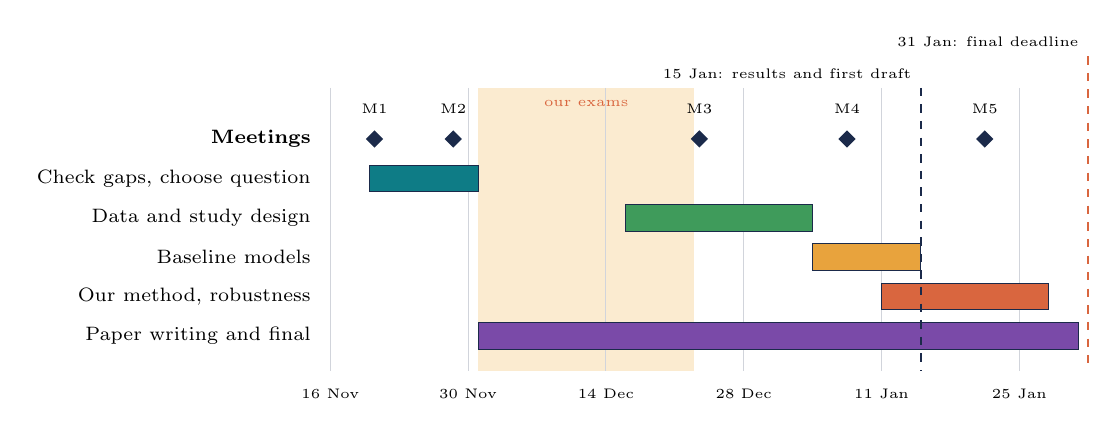
\begin{tikzpicture}[x=0.125cm,y=-0.5cm,font=\scriptsize]
\fill[softamber] (15,-1.3) rectangle (37,5.9);
\node[font=\tiny,text=coral] at (26,-0.9) {our exams};
\foreach \x/\l in {0/16 Nov,14/30 Nov,28/14 Dec,42/28 Dec,56/11 Jan,70/25 Jan}{
  \draw[navy!20] (\x,-1.3) -- (\x,5.9);
  \node[anchor=north,font=\tiny] at (\x,6.1) {\l};
}
\node[anchor=east] at (-1,0) {\textbf{Meetings}};
\node[anchor=east] at (-1,1) {Check gaps, choose question};
\node[anchor=east] at (-1,2) {Data and study design};
\node[anchor=east] at (-1,3) {Baseline models};
\node[anchor=east] at (-1,4) {Our method, robustness};
\node[anchor=east] at (-1,5) {Paper writing and final};
\filldraw[fill=teal,draw=navy,line width=0.3pt] (4,0.66) rectangle (15,1.34);
\filldraw[fill=leaf,draw=navy,line width=0.3pt] (30,1.66) rectangle (49,2.34);
\filldraw[fill=amber,draw=navy,line width=0.3pt] (49,2.66) rectangle (60,3.34);
\filldraw[fill=coral,draw=navy,line width=0.3pt] (56,3.66) rectangle (73,4.34);
\filldraw[fill=plum,draw=navy,line width=0.3pt] (15,4.66) rectangle (76,5.34);
\foreach \x/\l in {4.5/M1,12.5/M2,37.5/M3,52.5/M4,66.5/M5}{
  \node[diamond,fill=navy,inner sep=1.6pt] at (\x,0) {};
  \node[anchor=south,font=\tiny] at (\x,-0.4) {\l};
}
\draw[dashed,thick,navy] (60,-1.3) -- (60,5.9);
\node[anchor=south east,font=\tiny] at (60,-1.3) {15 Jan: results and first draft};
\draw[dashed,thick,coral] (77,-2.1) -- (77,5.9);
\node[anchor=south east,font=\tiny] at (77,-2.1) {31 Jan: final deadline};
\end{tikzpicture}

\vspace{1pt}
{\tiny M1: 20 Nov \;|\; M2: about 26--30 Nov \;|\; M3: about 23 Dec \;|\; M4: about 7 Jan \;|\; M5: about 21 Jan. Dates are tentative and depend on your availability.}

\vspace{3pt}
\noindent\colorbox{softteal}{\parbox{0.96\textwidth}{\scriptsize\raggedright\textbf{\color{teal}Why:} In exams (1--22 December) we work in a light mode. Experiments are frozen on 23 January, so writing and checking get enough time.}}
\end{frame}

% ------------------------------------------------------------ 24 EXPECTED IMPACT
\begin{frame}[t]{Expected impact}
\begin{columns}[T]
\column{0.32\textwidth}
\textbf{\color{teal}For research}\\[3pt]
Clear evidence on whether ESG uncertainty, disagreement or greenwashing text carries useful information, tested on later years, with honest reporting of what does not work.
\column{0.32\textwidth}
\textbf{\color{coral}For practice}\\[3pt]
Investors and banks could see an ESG score together with its reliability, and know how much to trust it.
\column{0.32\textwidth}
\textbf{\color{plum}For our team}\\[3pt]
A full paper draft and clean, reusable code by 31 January, and real research experience under your guidance.
\end{columns}
\vspace{10pt}
\why{If the results are positive, we add a useful tool. If they are negative, we still help the field by showing what does not work.}
\end{frame}

\section{Discussion}
% ------------------------------------------------------------ 25 QUESTIONS FOR PROFESSOR
\begin{frame}[t]{Questions for you}
\small
\begin{enumerate}
\setlength{\itemsep}{5pt}
\item Which of the eight research questions, or which bundle, do you find most promising?
\item Can we use Orbis? Which countries, sectors and years, and does it include ESG data? Are there download limits?
\item How could we connect our work to your ESG-washing research, and where can we get report text?
\item What kind of output are you aiming for (journal or conference), and what is realistic by 31 January?
\item What are the best dates for our next meetings (around 26--30 November and about 23 December)? Are you available around Christmas?
\item Could you suggest two or three introductory finance readings for computer science students?
\end{enumerate}
\end{frame}

% ------------------------------------------------------------ 26-27 REFERENCES
\begin{frame}[t]{References (1/2)}
\tiny
\setlength{\parskip}{3pt}
Avramov, Cheng, Lioui, and Tarelli (2022). Sustainable investing with ESG rating uncertainty. \emph{Journal of Financial Economics}, 145(2), 642--664. doi:10.1016/j.jfineco.2021.09.009

Berg, K\"olbel, and Rigobon (2022). Aggregate confusion: The divergence of ESG ratings. \emph{Review of Finance}, 26(6), 1315--1344. doi:10.1093/rof/rfac033

Calamai, Balalau, Le Guenedal, and Suchanek (2025). Detecting greenwashing: A natural language processing literature survey. arXiv:2502.07541 (preprint, v2 January 2026).

Caprioli et al.\ (2024). Denoising ESG: Quantifying data uncertainty from missing data with machine learning and prediction intervals. arXiv:2407.20047 (preprint).

Cheng, Cheong, Wojewodzki, and Chui (2025). The effect of ESG divergence on the financial performance of Hong Kong-listed firms: An artificial neural network approach. \emph{Research in International Business and Finance}, 73, 102616. doi:10.1016/j.ribaf.2024.102616

Del Vitto, Marazzina, and Stocco (2023). ESG ratings explainability through machine learning techniques. \emph{Annals of Operations Research}. doi:10.1007/s10479-023-05514-z

Dossa, Ukwuoma, Thomas, Dossa, and Gopang (2025). Prediction of nexus among ESG disclosure and firm performance: Applicability, explainability and implications. \emph{Innovation and Green Development}, 4(4).

Giudici and Wu (2025). Sustainable artificial intelligence in finance: impact of ESG factors. \emph{Frontiers in Artificial Intelligence}, 8, 1566197. doi:10.3389/frai.2025.1566197
\end{frame}

\begin{frame}[t]{References (2/2)}
\tiny
\setlength{\parskip}{3pt}
Lin and Hsu (2023). Empirical study of ESG score prediction through machine learning: A case of non-financial companies in Taiwan. \emph{Sustainability}, 15(19), 14106.

Liu, Li, and Yu (2025). Predicting financial distress with ESG-driven deep learning and risk-based stratification. \emph{International Journal of Finance and Economics}. doi:10.1002/ijfe.70077

Raza, Zaidi, and Thalassinos (2026). Do ESG scores and controversies improve corporate financial distress prediction? Evidence from machine learning in Asia-Pacific markets. \emph{European Research Studies Journal}, 29(2), 485--512. doi:10.35808/ersj/4380

Schimanski et al.\ (2024). Bridging the gap in ESG measurement: Using NLP to quantify environmental, social, and governance communication. \emph{Finance Research Letters}, 61, 104979. doi:10.1016/j.frl.2024.104979

UK greenwashing study (2026). Artificial intelligence models for detecting greenwashing in UK ESG and green finance projects. Zenodo record 18464861, published 31 January 2026 (independent researchers; not clearly peer reviewed).

Wu et al.\ (2025). Navigating ESG rating divergence: Implications for labor investment efficiency and firm adaptation strategy. \emph{Global Finance Journal}, 67, 101141. doi:10.1016/j.gfj.2025.101141

Zhang and Zhao (2026). Corporate ESG rating prediction based on XGBoost-SHAP interpretable machine learning model. \emph{Expert Systems with Applications}, 295, 128809. doi:10.1016/j.eswa.2025.128809

Zhao, Kroher, Engler, and Schnattinger (2023). Detecting greenwashing in the environmental, social, and governance domains using natural language processing. \emph{Proc.\ 15th International Joint Conference on Knowledge Discovery, Knowledge Engineering and Knowledge Management (KDIR)}, 175--181. doi:10.5220/0012155400003598
\end{frame}

% ------------------------------------------------------------ 28 CLOSING
\begin{frame}[plain]
\vspace{1.8cm}
\begin{center}
{\Huge\bfseries\color{navy}Questions and discussion}\\[10pt]
{\color{amber}\rule{6cm}{1.2pt}}\\[10pt]
{\Large Thank you, Professor Lagasio}\\[14pt]
{\normalsize\bfseries Rajnish Singh \;$\cdot$\; Medhavie Gupta \;$\cdot$\; Katyayani Jaiswal}
\end{center}
\end{frame}

\end{document}
